\documentclass[xcolor=dvipsnames]{beamer}


\usepackage[T1]{fontenc}
\usepackage[utf8]{inputenc}


\usepackage[french]{babel}
\usepackage{graphicx}%@@final
\usepackage{hyperref}
\usepackage{amsmath}
\usepackage{listings}
\usepackage{diagbox}
\usepackage{tikz}
\usetikzlibrary{shapes} 
\usepackage{xcolor}
\usepackage{url}
\usepackage{array}
 
 
\lstset{tabsize=2, numbers=left, numberstyle=\tiny, stepnumber=5, numbersep=5pt,breaklines=true,
    emph={int}, emphstyle=\color{red},
    emph={[2]int,for}, emphstyle={[2]\color{red}},
    emph={[3]int,for,printf}, emphstyle={[3]\color{blue}},
    morecomment=[s][\color{green}]{/*}{*/}
}
 
\newcolumntype{P}[1]{>{\centering\arraybackslash}p{#1}} 
 
 
\usetheme{Pittsburgh}
%\setbeamercovered{invisible}  
%\useinnertheme[shadow=true]{rounded}
%\useoutertheme{infolines}
\usecolortheme{dove}
\setbeamerfont{block title}{size={}}
\setbeamercolor{titlelike}{parent=structure,bg=white} 
\setbeamercolor{item}{fg=RedOrange}

\setbeamertemplate{footline}[frame number]
 
\hypersetup{%colorlinks,%
%citecolor=black,%
%filecolor=black,%
%linkcolor=black,%
urlcolor=red}
 
\author {Nicolas Paliod, Martin Chevalier,\\Lionel Delta, Thomas Deroyon}

\title{Gustave: An R \textit{package} \\ for variance estimation in surveys}
\institute{New Techniques and Technologies for Statistics 2019}

\AtBeginSection[]
 {
 \begin{frame}<beamer>
 \frametitle{Plan}
 \tableofcontents[sectionstyle = show/shaded,hideallsubsections]
 \setcounter{tocdepth}{1}
 \end{frame}
 }

\date{13 March 2019}

\begin{document}
\begin{frame}
\maketitle 
\begin{center}

\includegraphics[width=2cm]{logo.png}
\end{center}
\end{frame}

\section*{Introduction}

\begin{frame}{Why computing variance estimations of a survey indicator?}

\begin{itemize}
    \item Variance estimation is important \textcolor{red}{for the data analyst} :
    \begin{itemize}
        \vspace{0.1cm}
        \item Enables to get a confidence interval
        \vspace{0.1cm}
        \item Enables to comment variations' significance
    \end{itemize}
    
    \vspace{0.2cm}
    \item Variance estimation is a way to \textcolor{red}{measure survey indicators' quality}
    \begin{itemize}
        \vspace{0.1cm}
        \item Included in the quality reports sent to Eurostat
        \vspace{0.1cm}
        \item Required in different surveys by the new European framework regulation for household surveys (\textit{Integrated European social statistics}) under negotiation
    \end{itemize}
    
    \vspace{0.2cm}
   
    \item Variance estimation is an important step in the \textcolor{red}{production process of a survey}
\end{itemize}

\end{frame}


\begin{frame}{Goals}
   
What Gustave is supposed to do : 

    \vspace{0.1 cm}
    
    \begin{itemize}
        \item \textcolor{red}{Facilitates interactions} between methodologists and data analysts
       
        \vspace{0.1 cm}
        
        \item Offers a computational framework to methodologists and data analysts with \textcolor{red}{existing functionalities} (linearization functions, domains...)
         
        \vspace{0.1 cm}
        
        \item Simplifies \textcolor{red}{analytical variance estimation}
      
    \end{itemize}

    \vspace{0.5 cm}

What Gustave does not do : 
    
    \vspace{0.1 cm}

    \begin{itemize}
        \item Does not provide a ready for use variance estimation function to methodologists
       
        \vspace{0.1 cm}
        
        \item Does not offer a computational framework for variance estimation with bootstrap
    
    \end{itemize}

\end{frame}




\section{The use of Gustave}


\begin{frame}{A toolkit}

\begin{itemize}
    
    \item Variance estimation for domains included in Gustave
    
    \vspace{0.2 cm}
    
    \item Some linearization functions included in Gustave (\textit{ratio}, \textit{diff\_of\_ratio}, \textit{mean})
    
    \vspace{0.2 cm}

    \item Some variance functions already coded (Sen Yates Grundy variance estimator \textit{varSYG}, Deville-Tille variance estimator \textit{varDT})
    
    \vspace{0.2 cm}

    \item A way to take into account calibration included in the package (\textit{res\_cal})

\end{itemize}
    
\end{frame}



\begin{frame}{The use of Gustave for the methodologist}

What the methodologist produces:

\vspace{0.1 cm}

\begin{itemize}
    
    \item A variance function for a total
    
\end{itemize}

\vspace{0.5 cm}

What the methodologist does not need to code:

\vspace{0.1 cm}

\begin{itemize}
    
    \item Formatting
    
    \vspace{0.1 cm}

    \item Estimation for domains
    
    \vspace{0.1 cm}
    
    \item Classic linearization functions

\end{itemize}
       
\end{frame}


\begin{frame}{Example (1/2)}
    
\begin{itemize}
    \item \textcolor{red}{First step:} Data computation in order to prepare all variables which are necessary for the variance estimation (for instance, non-response units' probability)
    \vspace{0.5 cm} 
    \item \textcolor{red}{Second step:} Coding of the variance function \\ \textcolor{red}{Example} with a two-stage sample scheme with primary units' sampling before a dwellings' sampling, a reweighting for nonresponse adjustment and a calibration on simulated data of Labour Force Survey

\end{itemize}

\begin{center}
    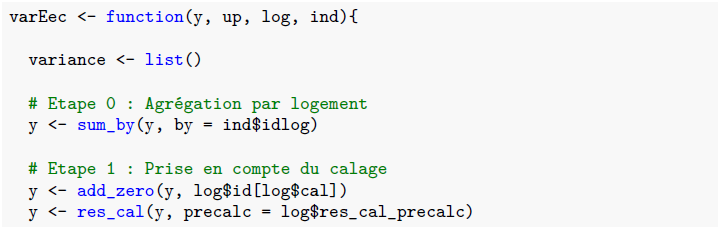
\includegraphics[width = 10 cm]{EEC_1.png}
\end{center}    

\end{frame}

\begin{frame}{Example (2/2)}
    
\begin{center}
    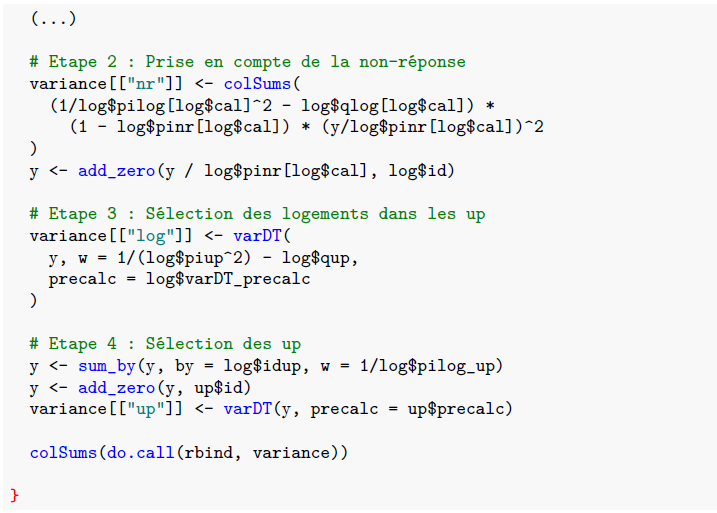
\includegraphics[width = 10 cm]{EEC_2.png}
\end{center}

\end{frame}




\begin{frame}{A key functionality: the variance \textit{wrapper} (1/2)}

The \textcolor{red}{variance wrapper adds functionalities} (linearization functions, estimation for domains, ...) to the variance function for totals coded by the methodologist

\vspace{0.5cm}

Last part of the example:
\begin{center}
    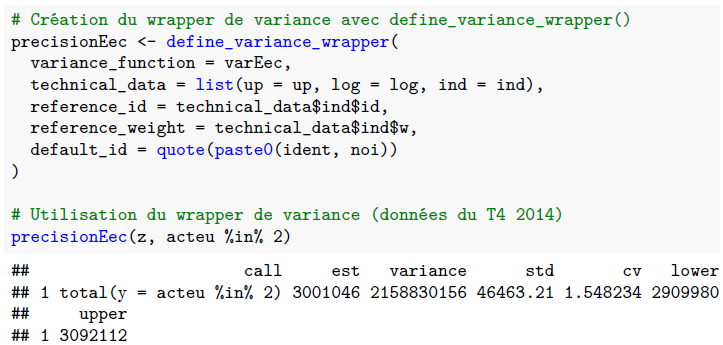
\includegraphics[width = 10 cm]{EEC_3.png}
\end{center}

\end{frame}


\begin{frame}{A key functionality: the variance \textit{wrapper} (2/2)}

Variance estimation of unemployment \textcolor{red}{rate}:
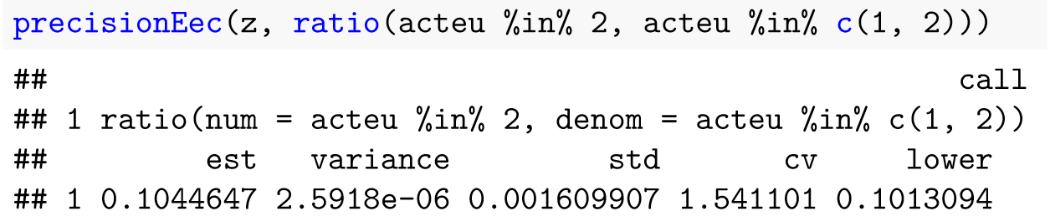
\includegraphics[width = 7 cm]{EEC_5.png}

\vspace{0.1 cm} 

Variance estimation of unemployment rate for people \textcolor{red}{over 50}:
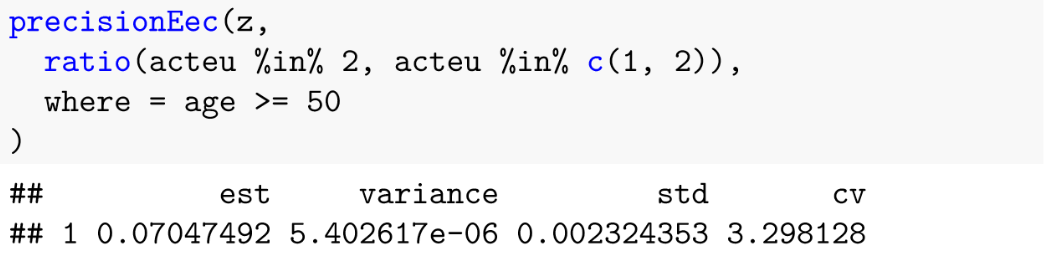
\includegraphics[width = 7 cm]{EEC_6.png}

\vspace{0.1 cm} 
Variance estimation of unemployment rate \textcolor{red}{by region}:
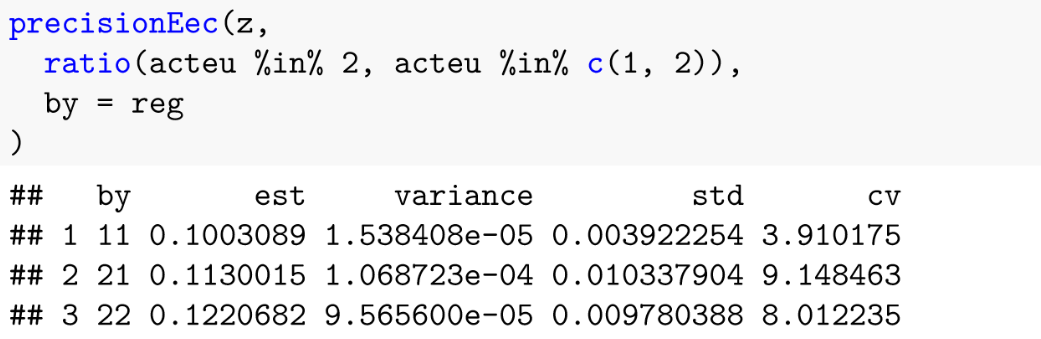
\includegraphics[width = 7 cm]{EEC_7.png}


\end{frame}


\begin{frame}{An expandable \textit{package}}

define\_variance\_wrapper() can handle \textcolor{red}{any variance function in input}: 
\vspace{0.2cm}
\begin{itemize}
    \item as many parameters as necessary for the variance function
    \vspace{0.1 cm}
    \item use of other \textit{packages} to code the variance function (use of require() in the variance function)
\end{itemize}

\vspace{0.2cm}

\textcolor{red}{New linearization functions} with define\_statistic\_wrapper() :

\begin{center}
    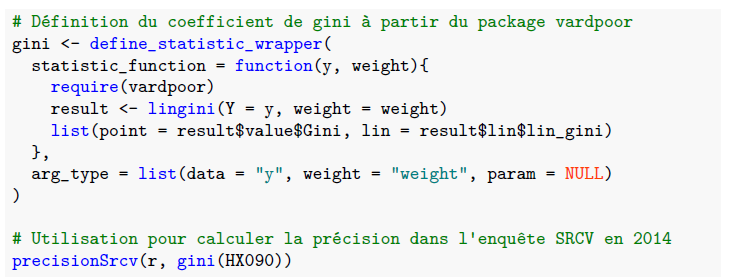
\includegraphics[width = 10 cm]{gini.png}
\end{center}    

\end{frame}







\begin{frame}{qvar(): a ready for use variance estimation function}

\begin{itemize}
    
    \item "What Gustave does not do: to provide a ready for use variance estimation function to methodologists"... but for \textcolor{red}{one specific case}

    \vspace{0.3 cm}

    \item \textcolor{red}{A ready for use variance estimation function} for the following case:
        \begin{itemize}
            \item Stratified simple random sampling
            \vspace{0.1 cm}
            \item Nonresponse adjustment by reweighting with response homogeneity groups
            \vspace{0.1 cm}
            \item Calibration
        \end{itemize}    
    
    \vspace{0.3 cm}
    
    \item Useful for business surveys
    
    \vspace{0.3 cm}

    \item qvar() built as a variance estimation function, which is integrated in a wrapper


\end{itemize}
    
\end{frame}


\begin{frame}{Dissemination at Insee}

Examples of use at Insee: 
    \vspace{0.2 cm}
    \begin{itemize}
        \item Labour Force Survey
        \vspace{0.1cm}
        \item Statistics on Income and Living Conditions
        \vspace{0.1cm}
        \item Some business surveys
    \end{itemize}


\vspace{0.4 cm}

Used for surveys with different issues: 
\vspace{0.2cm}
\begin{itemize}
    \item French master sample (household surveys, formula from Breidt, Chauvet, 2011 and Gros, Moussallam, 2015)
    \vspace{0.1cm}
    \item Multiple stages for indicators on individuals (Cadre de vie et sécurité)
    \vspace{0.1cm}
    \item Weight sharing (SILC)
\end{itemize}

\end{frame}


\section{Dissemination and developments}


\begin{frame}{Constraints for dissemination}

\begin{itemize}
    \item \textcolor{red}{Warning concerning the dissemination of the variance function produced in Gustave:} \\ \vspace{0.2 cm} The variance \textit{wrapper} is a fully self-sufficient function : answers to the survey and information describing the sample scheme are given in input in the technical\_data parameter and are  kept in the function environment (it's a \textit{closure})
    
    \vspace{0.5cm}

    \item \textcolor{red}{Be careful to disseminate the variance function only to people who have the right to access your data and are aware of the rules on confidentiality}
\end{itemize}

\end{frame}



\begin{frame}{Dissemination, unit testing and seamless integration}

\begin{itemize}
    \item \textit{package} available on \underline{\href{https://cran.r-project.org/web/packages/gustave/index.html}{\textcolor{red}{Cran}}}, last version: August 2018
    \vspace{0.5 cm}
    
    \item \textcolor{red}{Open source code} on several development platforms, in particular \underline{\href{https://github.com/martinchevalier/gustave}{github.com}}

    \vspace{0.5 cm}

    \item possibility for users to suggest \textcolor{red}{upgrades} (to rectify bugs, to answer to specific requests, \textit{pull requests})

    \vspace{0.5 cm}
    
    \item More than \textcolor{red}{180 unitary tests} in Gustave to test Gustave's functionalities
  
    \vspace{0.5 cm}

    \item Tests which are automatically computed at each \textit{package's} new version: \textcolor{red}{seamless integration}
\end{itemize}
    
\end{frame}


\section*{Conclusion}

\begin{frame}{Conclusion}

Insee's Statistical Method Department developed an R \textit{package} to \textcolor{red}{simplify variance estimation}:
\vspace{0.1 cm}
\begin{itemize}
    \item a solution that simplify methodologists' work
    \vspace{0.1 cm}
    \item production of variance estimation functions which are simple to use
    \vspace{0.1 cm}
    \item a documented \textit{package}, with a vignette in progress
\end{itemize}

\vspace{0.5 cm}

A \textit{package} \textcolor{red}{used for Insee's household surveys}:
\begin{itemize}
    \vspace{0.1 cm}
    \item to produce variance estimation joined to quality reports
    \vspace{0.1 cm}
    \item to check that surveys satisfy to IESS's precision constraints
\end{itemize}

\end{frame}

\end{document}
